% !TEX TS-program = pdflatex
% !TeX encoding = UTF-8
% !TeX spellcheck = en_GB

\documentclass[aspectratio=43]{beamer}
% use this instead for 16:9 aspect ratio:
%\documentclass[aspectratio=169]{beamer}
% supported acpect ratios  1610  169 149 54 43 (default) 32

\usepackage[english]{babel} 
\usepackage[utf8]{inputenc}
\usepackage[T1]{fontenc}
\usepackage{algorithm,algorithmic}
\usepackage{hyperref}
\usepackage{multimedia}
\usepackage{animate}
\usetheme{ETHbeamer}
\useinnertheme{rectangles}

\colorlet{ETHcolor1}{ETHa}
\colorlet{ETHcolor2}{ETHa}

\author{Beat Hubmann}

\title{CSE Case Studies Seminar\\
    S. Kirkpatrick et al.:\\	   
	Optimization by Simulated Annealing}

\date{March 12, 2020}

% uncomment if you do not want to use a department logo
\deplogofalse

% to get section outlines
% \AtBeginSection[]
% {
%   \begin{frame}
%     \frametitle{Outline}
%     \tableofcontents[currentsection,hideothersubsections]
%   \end{frame}
% }

% \AtBeginSubsection[]
% {
%   \begin{frame}
%     \frametitle{Outline}
%     \tableofcontents[currentsection,currentsubsection]
%   \end{frame}
% }

\begin{document}

\titleframe

% \begin{frame}
% 	\frametitle{Contents}
% 	\tableofcontents
% \end{frame}

\section{Introduction}

\begin{frame}
	% \frametitle{Title}
	\begin{center}	
		\begin{tikzpicture}
			\node<1->[anchor=south west, inner sep=0] (image) at (0,0) {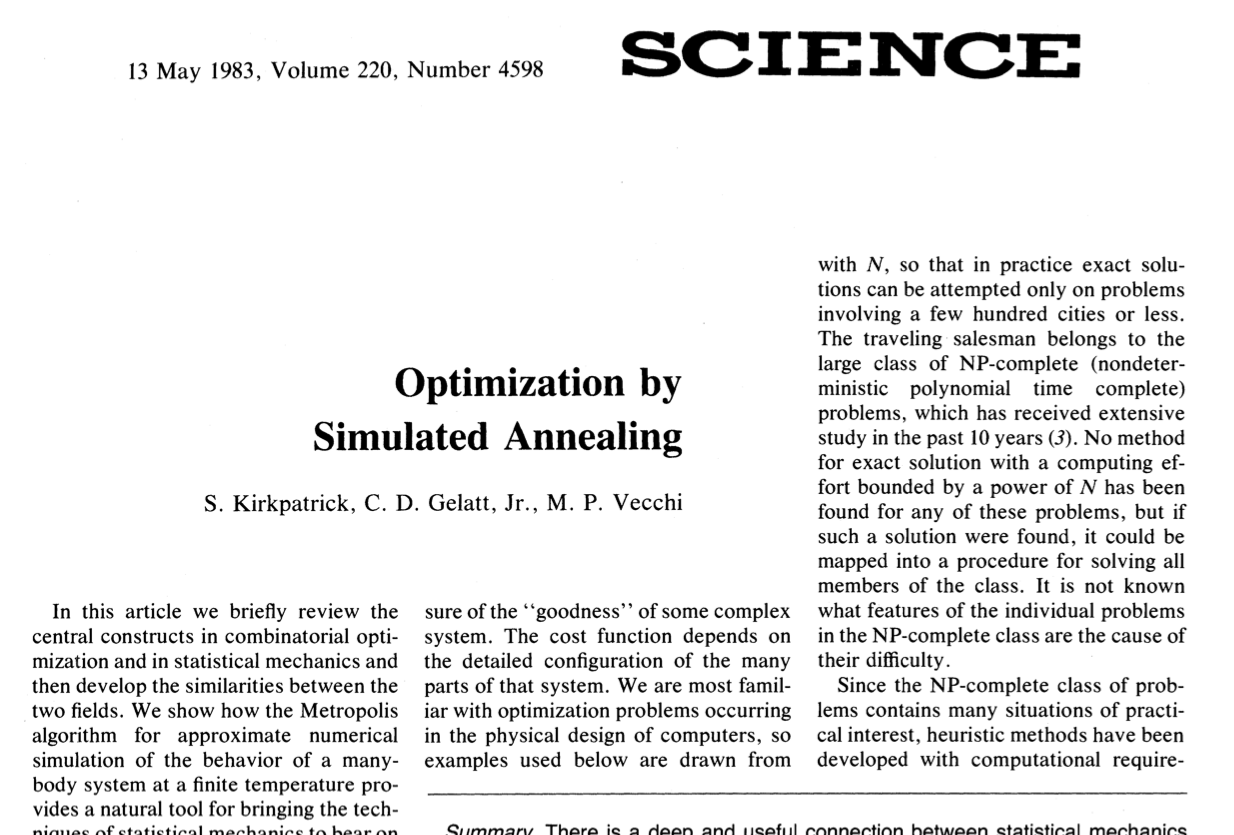
\includegraphics[height=7cm]{cover.png}};
			\draw<2-> [red, thick] (0.9, 6.2) rectangle (2.2, 6.75);
			% \node<2> [align=center, red, font={\Huge}] at (image.center) {ambiguous};
			% \node<3->[anchor=south west, inner sep=0] (image) at (0,0) {\includegraphics[height=5cm]{inverse_problems2.png}};
		\end{tikzpicture}\cite{Kirkpatrick}
	\end{center}
\end{frame}

\begin{frame}
% \frametitle{Title}
	\begin{center}	
		\begin{tikzpicture}
			\node<1->[anchor=south west, inner sep=0] (image) at (0,0) {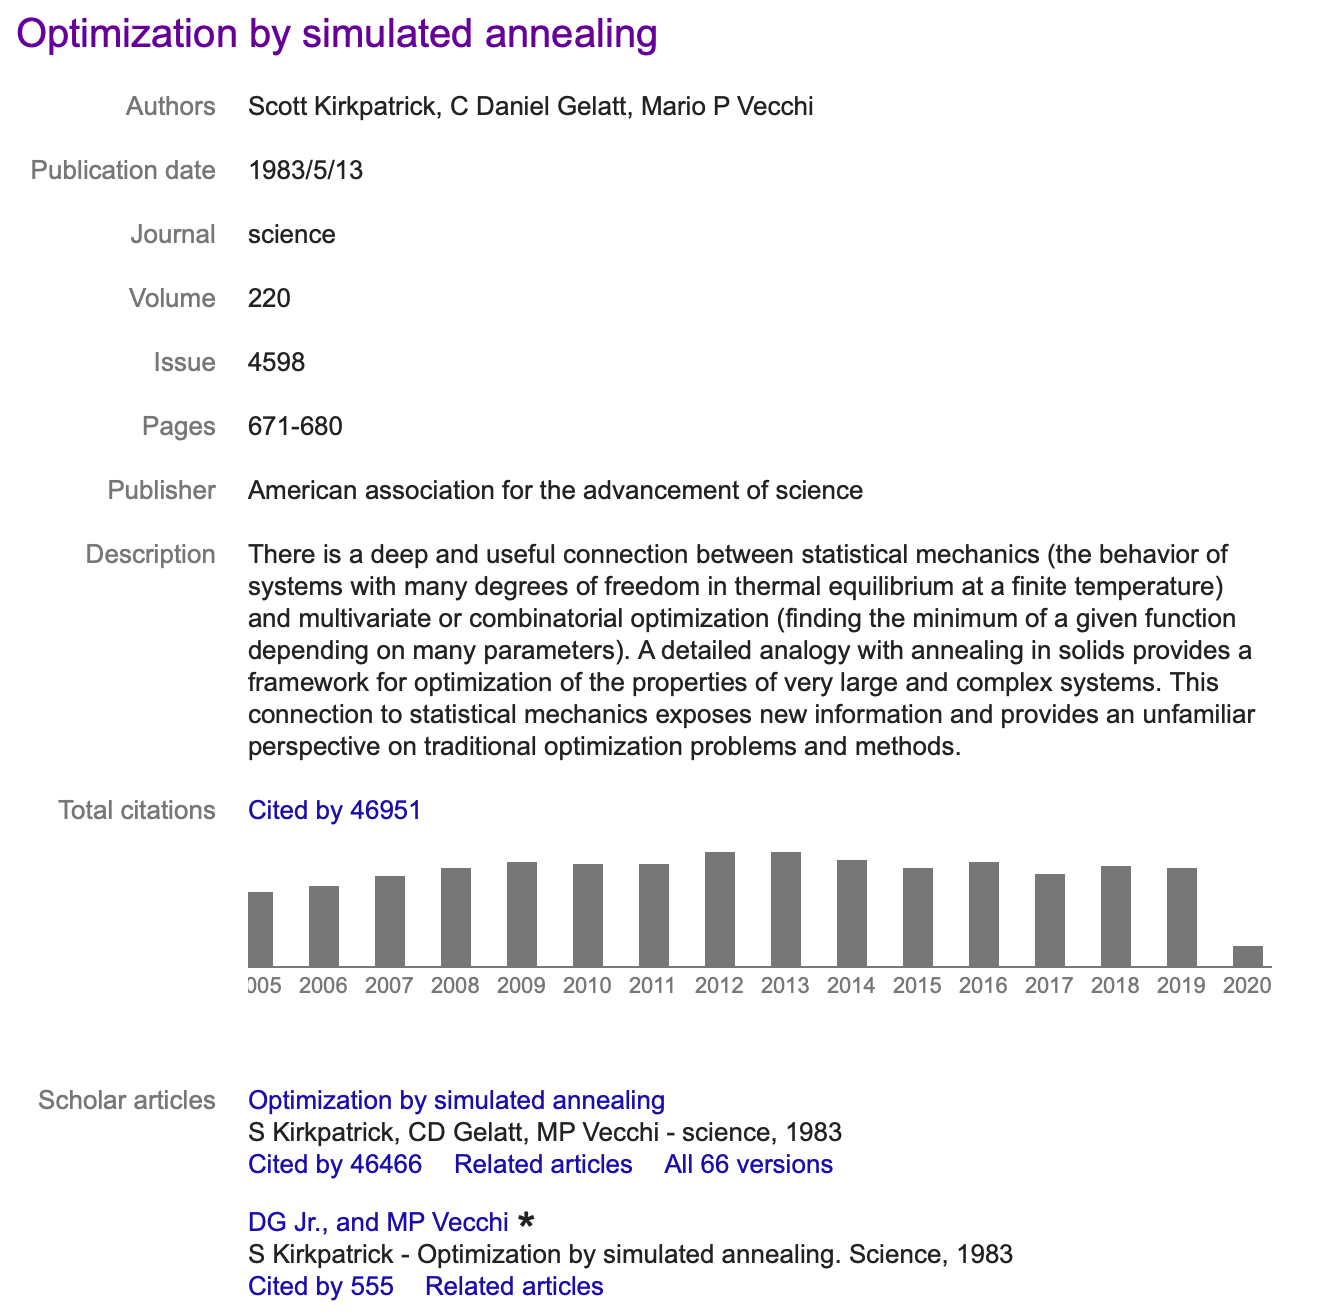
\includegraphics[height=9cm]{citations.png}};
			\draw<2-> [red, thick] (1.6, 2) rectangle (8.9, 3.7);
		\end{tikzpicture}\cite{GoogleScholar}
	\end{center}
\end{frame}



\section{Main subject}

\begin{frame}
	 \frametitle{Combinatorial optimization}
	 \begin{columns}[T]
		\begin{column}{0.5\textwidth}
			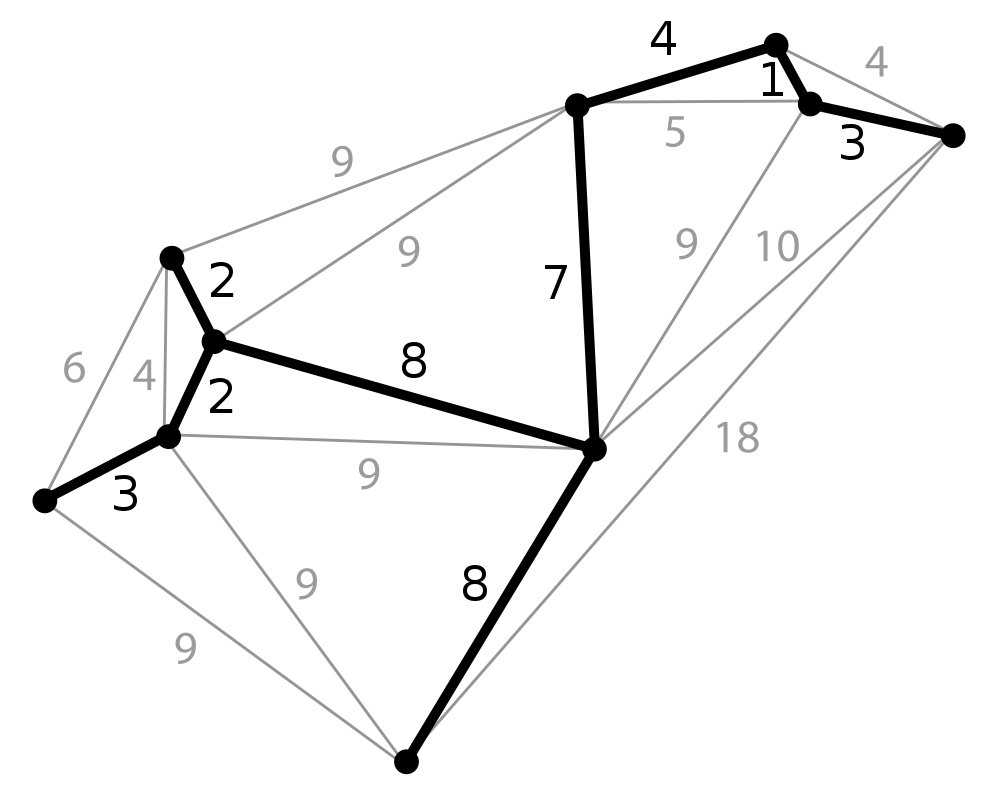
\includegraphics[width=5cm]{spanning_tree.png}\cite{Dcoetzee}	
		\end{column}
		\begin{column}{0.5\textwidth}
			\begin{itemize}
				\item finding optimum of function of \alert{'very many'} independent discrete variables
				\item in many cases, exhaustive search \alert{not tractable}
				\item often \alert{NP-hard}
			\end{itemize}
		\end{column}
	\end{columns}
\end{frame}

\begin{frame}
	 \frametitle{Example case 1: Chip design}
	 \begin{columns}[T]
		\begin{column}{0.5\textwidth}
			\begin{itemize}
				\item circuit placement
				\item wiring routes
				\item in general \alert{NP-hard}
			\end{itemize}	
		\end{column}
		\begin{column}{0.5\textwidth}
			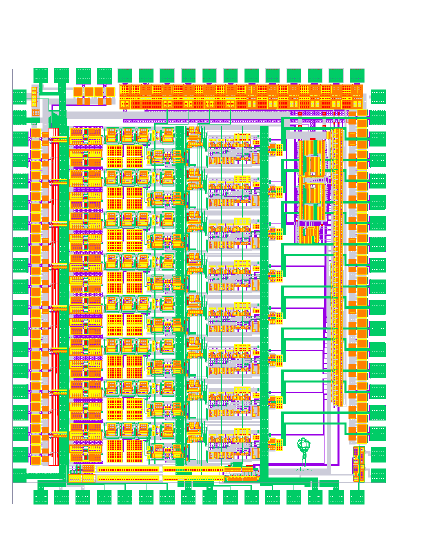
\includegraphics[width=5cm]{floor_plan.png}\cite{Pipino}				
		\end{column}
	\end{columns}
\end{frame}

\begin{frame}
	\frametitle{Example case 2: \alert{T}ravelling \alert{S}alesperson \alert{P}roblem}
	\begin{columns}[T]
		\begin{column}{0.5\textwidth}
			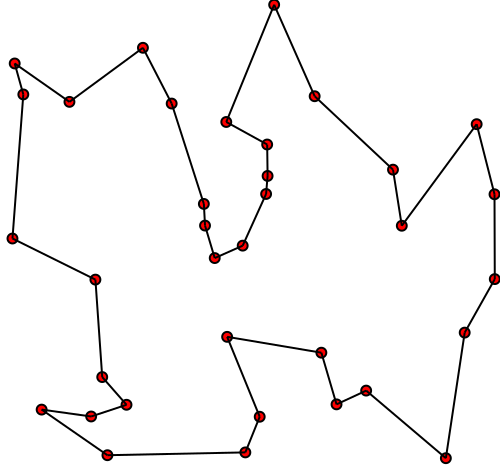
\includegraphics[width=5cm]{tsp.png}\cite{Xypron}
		\end{column}
		\begin{column}{0.5\textwidth}
			\begin{itemize}
				\item shortest possible route visiting each city and returning to origin
				\item generalized: \alert{vehicle routing problem (VRP)}
				\item \alert{NP-hard}
			\end{itemize}
		\end{column}			
	\end{columns}
\end{frame}

\begin{frame}
	\frametitle{TSP: Exact algorithms}
	\begin{itemize}
		\item<1-3> brute-force: $\mathcal{O}(n!)$
		\item<1-3> dynamic programming: $\mathcal{O}(n^2 2^n)$ (Held-Karp) 
		\item<2-> \alert{$\Rightarrow$ need heuristic methods:}
		\item<3> constructive heuristics
		\item<3> divide-and-conquer
		\item<3> iterative improvement
		\item<3-> randomized improvement
		\item<4-> \alert{$\quad \hookrightarrow$ simulated annealing}
	\end{itemize}
\end{frame}

\begin{frame}
	\frametitle{Simulated annnealing: Idea}
	\begin{itemize}
		\item<1-> inspired by condensed matter physics
		\item<1-> find ground state configuration in low temperature limit
		\item<2-> probability of state $x$: \alert{$P(x)\propto \exp(\frac{-E(x)}{k_BT})$}
		\item<2-> sample configuration space with MCMC: \alert{Metropolis}
		\item<3-> \alert{annealing schedule}: $\lim_{t \rightarrow t_\text{end}} T = 0$
	\end{itemize}
\end{frame}

\begin{frame}
	\frametitle{Molecular dynamics vs. TSP (1/4):\\\alert{System configuration description}}
	\begin{columns}[T]
		\begin{column}{0.5\textwidth}
			\begin{description}
				 \item<1-> phase space $\boldsymbol{r}=\{\vec{r_i}\}_{i \in N}$
			 \end{description}		
		\end{column}
		\begin{column}{0.5\textwidth}
			\begin{description}
				 \item<1-> tour as ordered list of vertices $\boldsymbol{T}=[1, 2, \ldots, N]$
			 \end{description}				
		\end{column}
	\end{columns}
\end{frame}

\begin{frame}
	\frametitle{Molecular dynamics vs. TSP (2/4):\\\alert{Random moves}}
	\begin{columns}[T]
		\begin{column}{0.5\textwidth}
			\begin{description}
				 \item<1-> randomly change one/several coordinates:\\ $\boldsymbol{r} \rightarrow \boldsymbol{r}'$
			 \end{description}
		\end{column}	
		\begin{column}{0.5\textwidth}
			\begin{description}
				 \item<1-> randomly swap two vertices:\\ $\boldsymbol{T} = [\ldots, 3, 7, 8,\ldots]$ $\rightarrow$ $\boldsymbol{T}'=[\ldots, 8, 7, 3,\ldots]$
			 \end{description}
		\end{column}			
	\end{columns}
\end{frame}

\begin{frame}
	\frametitle{Molecular dynamics vs. TSP (3/4):\\\alert{Quantitative objective function}}
	\begin{columns}[T]
		\begin{column}{0.5\textwidth}
			\begin{description}
				 \item<1-> $E \equiv$ Hamiltonian: $\mathcal{H}(\boldsymbol{r})$
			 \end{description}
		\end{column}		
		\begin{column}{0.5\textwidth}
			\begin{description}
				 \item<1-> $E \equiv$ Length of tour: $L(\boldsymbol{T})$
			 \end{description}
			\end{column}
	\end{columns}
\end{frame}

\begin{frame}
	\frametitle{Molecular dynamics vs. TSP (4/4):\\\alert{Acceptance probability and annealing}}
	\begin{center}
		\begin{description}
			\item<1-> Changed configuration acceptance probability \alert{$P_\text{acc} = \min(1, \exp(\frac{-\Delta E}{k_BT}))$}
			\item<2-> Annealing schedule \alert{$\lim_{t \rightarrow t_\text{end}} T = 0$}
		\end{description}
	\end{center}
\end{frame}



\section{Examples}

\begin{frame}
	\frametitle{Simulated annealing for 400-city TSP}
	\begin{center}
		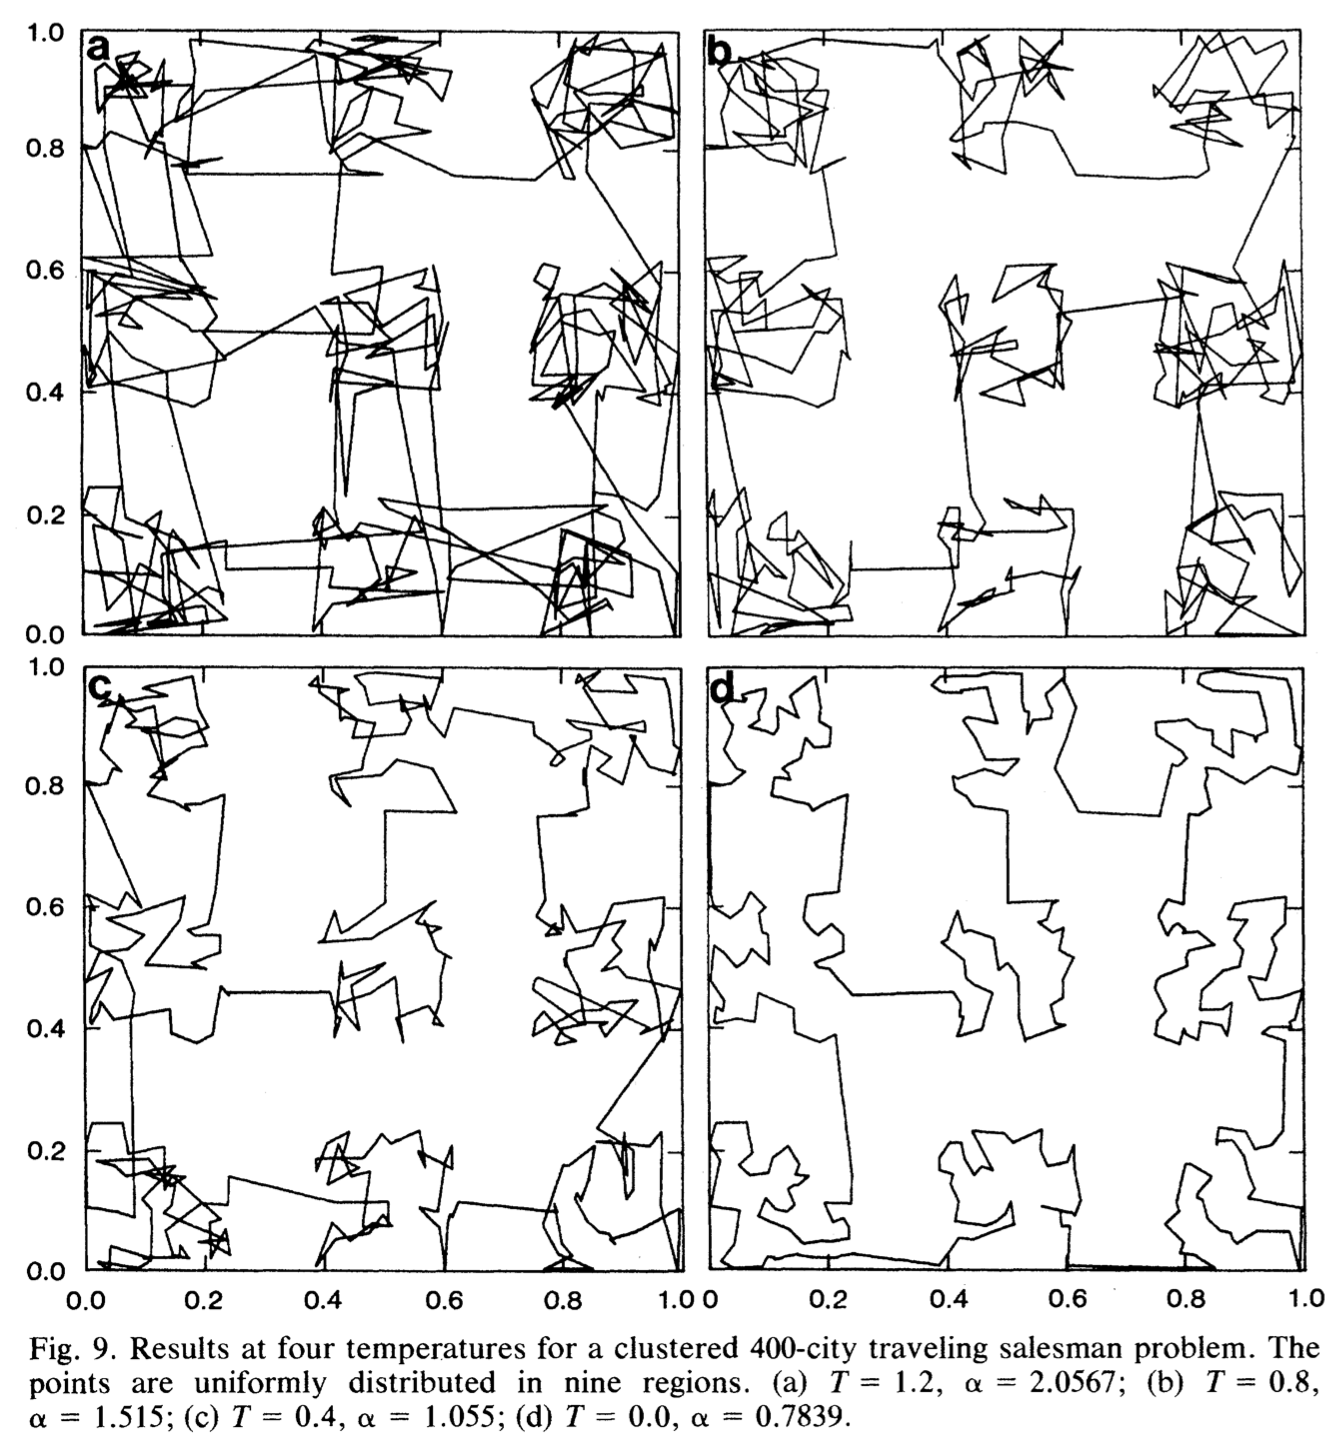
\includegraphics[width=6.8cm]{tsp_400.png}\cite{Kirkpatrick}
	\end{center}
\end{frame}

\begin{frame}
	\frametitle{Animated simulated annealing for 125-city TSP}
	\begin{center}
		\animategraphics[controls=all, height=6.6cm]{15}{tsp_simulated_annealing-}{0}{124}\cite{Geodac}
	\end{center}
\end{frame}

\begin{frame}
	\frametitle{Simulated annealing: The gist}
	\begin{center}
		\begin{itemize}
			\item<1-> \alert{'a balance between exploration and exploitation'}
			\item<1-> based on statistical mechanics
			\item<1-> improves iteratively, but has probabilistic component to avoid getting stuck in local minima
		\end{itemize}
	\end{center}
\end{frame}

\begin{frame}
	% \frametitle{Example}
	\begin{center}
		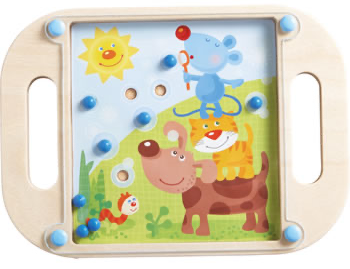
\includegraphics[width=6.8cm]{toy.png}
	\end{center}
\end{frame}

\section{Conclusion}

\begin{frame}
	\frametitle{Simulated annealing: Advantages}
	\begin{center}
		\begin{itemize}
			\item<1-> \alert{'decent enough'} approximate optimum in fixed amount of time
			\item<1-> well suited for discrete search spaces
			\item<1-> agnostic to system type, objective function
			\item<1-> relatively simple and independent of problem complexity to implement
		\end{itemize}
	\end{center}
\end{frame}

\begin{frame}
	\frametitle{Simulated annealing: Challenges}
	\begin{center}
		\begin{itemize}
			\item<1-> \alert{deciding set of moves and objective function} requires insight into problem and \alert{may not be obvious}
			\item<1-> \alert{annealing schedule} usually to be determined empirically
		\end{itemize}
	\end{center}
\end{frame}

\begin{frame}
	\frametitle{My conclusion}
	\begin{center}
		\begin{tikzpicture}
			\node<2->{
\includegraphics[width=5cm]{positive.png}};
		\end{tikzpicture}
	\end{center}

\end{frame}


\appendix
	\section*{References}
		\begin{frame}[allowframebreaks]
			\frametitle{References}
			\begin{thebibliography}{10}
				\bibliographystyle{apalike}

				% \beamertemplatebookbibitems
				% % Start with overview books.
			
				% \bibitem{Author1990}
				%   A.~Author.
				%   \newblock {\em Handbook of Everything}.
				%   \newblock Some Press, 1990.
				
				\beamertemplatearticlebibitems
				% Followed by interesting articles.
			
				\bibitem{Kirkpatrick}		
					S. Kirkpatrick et al.
					\newblock Optimization by Simulated Annealing.
					\newblock {\em science 220(4598), pp.571-680}, 1983
					\newblock \href{hhttps://www.jstor.org/stable/1690046}{DOI: 10.1126/science.220.4598.671}

				\bibitem{GoogleScholar}
					Google Scholar.
					\newblock Scott Kirkpatrick.		
					\newblock {\em Citation Profile}, \href{https://scholar.google.com/citations?user=qlKWTsUAAAAJ&hl=en&oi=sra}{Google Scholar (retrieved Mar 10, 2020)}

				\bibitem{Dcoetzee}
					User Dcoetzee.
					\newblock File:Minimum spanning tree.svg
					\newblock {\em Public Domain}, \href{https://commons.wikimedia.org/wiki/File:Minimum_spanning_tree.svg}{Wikimedia Commons (retrieved Mar 10, 2020)}

				\bibitem{Pipino}
					A. Pipino et al.
					\newblock sMDT Detectors Read-Out in 28nm technology.
					\newblock {\em IEEE International Conference on Electronics conference paper}, \href{https://www.researchgate.net/publication/338795012_sMDT_Detectors_Read-Out_in_28nm_technology}{DOI: 10.1109/ICECS46596.2019.8964714},
					2019.

				\bibitem{Xypron}
					User Xypron.
					\newblock File:GLPK solution of a travelling salesman problem.svg
					\newblock {\em Public Domain}, \href{https://commons.wikimedia.org/wiki/File:GLPK_solution_of_a_travelling_salesman_problem.svg}{Wikimedia Commons (retrieved Mar 10, 2020)}

				\bibitem{Geodac}
					User Geodac.
					\newblock File:Travelling salesman problem solved with simulated annealing.gif
					\newblock {\em Creative Commons CC0 1.0}, \href{https://commons.wikimedia.org/wiki/File:Travelling_salesman_problem_solved_with_simulated_annealing.gif}{Wikimedia Commons (retrieved Mar 10, 2020)}
			\end{thebibliography}
		\end{frame}
\end{document}
